\documentclass[12pt,letterpaper]{report}

% SENG 4130 Software Design Patterns report template (Fall 2026).
% Build with latexmk -pdf main.tex from this directory.

\usepackage[letterpaper,margin=1in]{geometry}
\usepackage[T1]{fontenc}
\usepackage[utf8]{inputenc}
\usepackage{lmodern}
\usepackage{microtype}
\usepackage{graphicx}
\usepackage{booktabs}
\usepackage{tabularx}
\usepackage{array}
\usepackage{longtable}
\usepackage[table]{xcolor}
\usepackage{enumitem}
\usepackage{caption}
\usepackage{float}
\usepackage{setspace}
\usepackage{titlesec}
\usepackage[hidelinks]{hyperref}
\usepackage[nameinlink,noabbrev]{cleveref}
\usepackage{fancyhdr}
\usepackage{etoolbox}

\definecolor{PromptGray}{HTML}{555555}
\definecolor{TableHeader}{HTML}{D9EAF7}
\definecolor{TableStripe}{HTML}{F4F7F9}
\renewcommand{\arraystretch}{1.25}
\setlength{\parindent}{0pt}
\setlength{\parskip}{0.65em}
\setcounter{secnumdepth}{3}
\setcounter{tocdepth}{3}
\titleformat{\chapter}{\normalfont\huge\bfseries}{\thechapter}{0.8em}{}
\titlespacing*{\chapter}{0pt}{-20pt}{18pt}

% Fill in the team and submission details when preparing each deliverable.
\newcommand{\projecttitle}{HAL -- Home Automation Layer}
\newcommand{\coursename}{SENG 4130 -- Software Design Patterns}
\newcommand{\submissiondate}{Date submitted}
\newcommand{\teammembers}{%
  Isaac Latta (T00239008)\\
}

% Enable once references.bib contains sources cited with \cite{key}.
\newif\ifreportreferences
\reportreferencestrue
\renewcommand{\bibname}{References}
% Match the supplied template's numbered References chapter.
\patchcmd{\thebibliography}{\chapter*{\bibname}}{\chapter{\bibname}}{}{
  \PackageError{hal-report}{Could not number the bibliography heading}{}
}

% Template instructions are visibly distinct and easy to remove as sections are written.
\newcommand{\templateprompt}[1]{%
  \begin{quote}\color{PromptGray}\itshape #1\end{quote}%
}

\newcommand{\placeholderfigure}[2]{%
  \begin{figure}[H]
    \centering
    \fbox{\parbox[c][2.0in][c]{0.82\textwidth}{\centering #1}}
    \caption{#2}
  \end{figure}
}

\newcommand{\meetingtemplate}[1]{%
  \section{Meeting #1}
  \textbf{Time:} Date and time to be recorded.\\
  \textbf{Agenda:} To be recorded.
  \begin{table}[H]
    \centering
    \caption{Meeting #1 task distribution and progress}
    \begin{tabularx}{\textwidth}{X X X X}
      \rowcolor{TableHeader}
      \textbf{Team Member} & \textbf{Previous Task} & \textbf{Completion State} & \textbf{Next Task} \\
      \hline
      Team member 1 & & & \\
      \rowcolor{TableStripe}Team member 2 & & & \\
    \end{tabularx}
  \end{table}
}

\pagestyle{fancy}
\fancyhf{}
\fancyfoot[C]{\projecttitle}
\fancyfoot[R]{\thepage}
\renewcommand{\headrulewidth}{0pt}

% Chapter-opening pages use the "plain" page style.
\fancypagestyle{plain}{
  \fancyhf{}
  \fancyfoot[C]{\projecttitle}
  \fancyfoot[R]{\thepage}
}

% Cover page: project name, without a page number.
\fancypagestyle{cover}{
  \fancyhf{}
  \fancyfoot[L]{\projecttitle}
}

\begin{document}

\hypersetup{pageanchor=false}
\begin{titlepage}
  \thispagestyle{cover}
  \centering
  
\includegraphics[width=\textwidth]{figures/tru-logo.png}\par
  \vspace{1.1in}
  {\Large\bfseries Department of Engineering\par}
  \vspace{0.5in}
  {\Large \coursename\par}
  {\large Fall 2026\par}
  \vspace{0.75in}
  {\Huge\bfseries \projecttitle\par}
  \vspace{0.8in}
  {\large \teammembers\par}
  \vfill
  {\large \submissiondate\par}
\end{titlepage}

\hypersetup{pageanchor=true}
\pagenumbering{roman}
\tableofcontents
\listoffigures
\listoftables
\clearpage
\pagenumbering{arabic}

% Deliverable 1 (October 6, 2026): Introduction, problem definition,
% scope, design requirements, and initial system design using UML.
% Later chapters remain as scaffolding for subsequent deliverables.
\chapter{Introduction}
Smart-home systems combine connected devices and sensors to support tasks such as controlling lighting, regulating temperature, and monitoring household security. Their use has grown: Statistics Canada's 2022 Canadian Internet Use Survey reported that the share of Canadians using Internet-connected smart-home devices increased from 42\% in 2020 to 47\% in 2022~\cite{statcan2023cius}. As these devices become more common, coordinating their behaviour and making their operation understandable become important software concerns. Earlier research illustrates the practical difficulties involved. Through visits to 14 households with home automation, Brush et al.~\cite{brush2011home} identified ownership costs, inflexibility, management difficulties, and security as barriers to adoption. Although this study describes an earlier generation of systems, it provides useful motivation for examining how residents configure and manage devices together. For this project, these concerns translate into a need for consistent monitoring, straightforward controls, and a system that can accommodate additional devices without extensive changes.

Research has addressed both the structure of smart-home software and the way users understand its behaviour. Dixon et al.~\cite{dixon2012an} proposed HomeOS, which represents networked home devices through abstract interfaces and allows applications to coordinate them through a common platform. This approach illustrates how separating device-specific details from application behaviour can support extension and reuse. However, providing a common interface does not by itself ensure that automation behaves as users expect. Huang and Cakmak~\cite{huang2015ubicomp} found that distinctions between event and state triggers, together with different types of actions, can lead to inconsistent interpretations and errors in trigger-action programs. For example, responding when a door opens differs from responding whenever a door is already open. These findings motivate attention to both software organization and precise behavioural requirements: users need to understand what causes an action, when it occurs, and how operating settings affect it.

HAL (Home Automation Layer) will explore these concerns through a Java Swing application for one simulated home. It will combine device monitoring, manual controls, and selected lighting, heating, security, and smoke-warning scenarios, with an Observe mode that retains monitoring without automatic actions or alerts. The following sections define the problem, scope, and requirements that will guide the subsequent software design and implementation.

\chapter{Design Problem}

\section{Problem Definition}
A home containing several smart devices needs a consistent way to monitor their states, control their operation, and respond to sensor input. These activities must work together: a sensor reading is useful only if the system can present it clearly and perform the appropriate action. The response may also depend on the user's selected operating mode. For example, motion while a resident is at home may require lighting, while motion when the resident is away may require a security warning.

HAL (Home Automation Layer) will address this problem through a desktop application that combines monitoring, manual control, and automatic responses for a simulated home. The primary user is a resident who needs to understand the home's current condition, control available devices, and select how the system responds to events. Simulation controls will allow these behaviours to be demonstrated without physical equipment.

The central problem is to coordinate different devices and sensors while keeping the system understandable and adaptable. Adding a device should not require rebuilding the application, and the loss of one device should not prevent unrelated devices from operating. The project will demonstrate these capabilities through a small set of repeatable home-automation scenarios.

\subsection{Scope}
The proposed scope is one simulated home operated through a Java Swing desktop interface. The initial device set will include smart lights, a thermostat, and a door lock, together with motion, temperature, door, and smoke sensors. Each device will have an identifiable name, a current state or reading, and an availability status. A door sensor will report whether the door is open or closed; this is separate from whether its lock is locked or unlocked.

The application will provide three operating modes: Home, Away, and Observe. In Observe mode, HAL will continue updating device states and sensor readings and recording events, but will issue no alerts and perform no automatic device actions. Manual controls will remain available. Entering Observe mode will hide active alerts without deleting their history and leave device states unchanged. Returning to Home or Away mode will resume automation and alert evaluation using current readings.

The application will support manual device control and four automatic behaviours in Home and Away modes:
\begin{itemize}[leftmargin=*]
  \item \textbf{Lighting:} In Home mode, detected motion will turn on an associated light.
  \item \textbf{Security:} In Away mode, detected motion or an opened door will produce a visible security warning.
  \item \textbf{Temperature control:} In Home and Away modes, temperature readings will determine whether simulated heating is active, using the target temperature for the selected Comfort or Energy-saving setting.
  \item \textbf{Smoke warning:} A smoke-detected event will produce a visible warning in either Home or Away mode.
\end{itemize}

Sensor updates will be generated periodically by the simulation and can also be triggered through the interface. The user will be able to add and remove instances of supported device types and simulate a device becoming unavailable. A session activity log will show sensor events, user actions, automatic responses, and failures.

The initial scope excludes physical hardware, commercial smart-home integrations, Internet remote access, mobile applications, video processing, and email or SMS notifications. Persistence between application runs and a user-defined automation rule editor are also outside the scope. HAL is an educational simulation, with warnings and device actions represented within the application.

\section{Design Requirements}
The following requirements describe the intended behaviour of the prototype and will guide implementation and demonstration. They do not indicate completed features. The selected device set, scenarios, and acceptance targets are proposed project requirements within the broader course brief.

\subsection{Functions}
\begin{enumerate}[label=\textbf{F\arabic*.},leftmargin=*]
  \item \textbf{Monitor the home.} Display each registered device's name, type, availability, and current state or reading. Show the operating mode and temperature setting. Display active warnings in Home and Away modes; in Observe mode, display readings and availability without issuing alerts.
  \item \textbf{Manage devices.} Allow the user to add and remove instances of supported device and sensor types. Removed devices must stop contributing readings or receiving actions.
  \item \textbf{Generate sensor input.} Provide periodic simulated updates while the simulation is running and controls for triggering specific inputs. Support motion detected/cleared, door opened/closed, smoke detected/cleared, and numerical temperature readings.
  \item \textbf{Control devices manually.} Allow the user to switch lights on or off, lock or unlock the simulated door lock, and adjust the thermostat target. Reflect successful changes in the displayed device state.
  \item \textbf{Select automation behaviour.} Allow the user to select Home, Away, or Observe mode and a Comfort or Energy-saving temperature setting. Apply the selected settings to subsequent events. The Energy-saving target must be lower than the Comfort target for the heating demonstration.
  \item \textbf{Respond automatically.} Perform the lighting, security, temperature, and smoke-warning behaviours defined in the scope. In Home and Away modes, activate simulated heating below the selected target and deactivate it at or above that target. In Observe mode, suppress all automatic device actions and alerts, including smoke, security, and device-failure alerts. Record automatic actions together with their triggering events.
  \item \textbf{Handle unavailable devices.} Allow availability to be changed during a demonstration. Mark unavailable devices clearly, stop using their readings as current input, and report actions that cannot be completed. In Home and Away modes, suspend automatic heating and show a warning if temperature input becomes unavailable. In Observe mode, update availability and log the failure without issuing an alert or changing device states automatically. Continue processing events for unaffected devices.
  \item \textbf{Report activity.} Maintain a time-ordered session log of sensor events, manual actions, automatic responses, and failures. Clear an active sensor warning when its corresponding clear event is received, while retaining its history in the log. Continue recording sensor events and failures in Observe mode without presenting them as alerts.
  \item \textbf{Restrict access.} Require successful sign-in before displaying home status or accepting control and configuration actions. Signing out must return the interface to the sign-in screen and prevent further access until the user signs in again.
\end{enumerate}

\subsection{Objectives}
\begin{description}[style=nextline]
  \item[Extensible and maintainable.]
  Additional device types should be supported without major changes to existing functionality. Assessment will consider the changes needed to add a device type and whether existing scenarios continue to work.
  \item[Usable and consistent.]
  States, readings, warnings, and controls should have clear labels and consistent presentation. A user should be able to inspect a device, change its state, select a mode, and identify a warning through the interface without editing code.
  \item[Reliable and robust.]
  Repeating a scenario with the same initial state, settings, and input should produce the same observable response. Invalid input and an unavailable device should not terminate the application or stop unrelated automation.
  \item[Responsive.]
  Events and manual actions should produce visible feedback promptly. The proposed acceptance target is feedback within one second of receiving an event or action, with ten registered simulated devices on the demonstration computer. This is a prototype target rather than a guarantee for physical control systems.
  \item[Flexible.]
  Users should be able to change modes and temperature settings during a session. Demonstrations will compare responses to the same sensor input under different settings without restarting the application.
  \item[Scalable within the project scope.]
  The application should handle multiple instances of supported device types. A demonstration with ten registered devices will check that their identities and states remain distinct and the interface remains responsive.
\end{description}

\subsection{Constraints}
These constraints have pass-or-fail checks. The first two record course requirements; the remaining constraints address engineering considerations for this prototype.
\begin{enumerate}[label=\textbf{C\arabic*.},leftmargin=*]
  \item \textbf{Implementation technology.} The application must use Java and a Java Swing graphical interface. All device and sensor behaviour must be simulated in software, with no physical smart-home hardware required.
  \item \textbf{Design patterns.} The completed system must apply at least five software design patterns. The report must justify their use and explain how they cooperate in an automation scenario. Specific patterns will be selected during the design stage.
  \item \textbf{Privacy.} Demonstration data must be synthetic. The application must not require real household records, camera footage, or personal information, and must not transmit simulated home activity to an external service.
  \item \textbf{Security.} An unsigned-in user must not be able to view home status, control devices, or change settings through the application. Failed sign-in attempts must leave those functions inaccessible. This will be checked before sign-in and again after sign-out.
  \item \textbf{Safety.} The interface must identify the system as a simulation. Smoke and security warnings must appear within the application only; no action may operate real equipment or contact emergency services.
  \item \textbf{Reliability.} When one device becomes unavailable, the application must remain running, identify that device, report any failed action involving it, and successfully process a subsequent event involving an unaffected device. An unavailable sensor's last reading must not be presented as current.
  \item \textbf{Economic feasibility.} The prototype must run on an existing development computer without purchasing smart-home equipment or requiring a paid cloud service or subscription.
\end{enumerate}

\chapter{Solution}
\templateprompt{Describe the alternatives considered and how the design evolves to satisfy the functions, objectives, and constraints. For deliverable one, present a proposed initial design; update the selected solution as the project develops. Record actual alternatives and decisions as they are made.}

\section{Solution 1}
\templateprompt{Describe the first design alternative, its strengths and weaknesses, and the reasons for retaining or rejecting it.}

\section{Solution 2}
\templateprompt{Describe an improved or alternative design and evaluate it against the requirements and constraints.}

% The Word template's body includes Solution 3, although its sample TOC omits it.
\section{Solution 3}
\templateprompt{Describe a further design alternative if considered, or remove this section if it is unnecessary.}

\section{Final Solution}
\templateprompt{Explain why the selected design is preferable to the alternatives, using a comparison table if useful. At the initial-design stage, clearly identify this as a proposed solution.}

\subsection{Features}
\templateprompt{Describe the selected features and the components, functions, or methods that support them. Distinguish planned features from implemented ones as the project progresses.}

\subsubsection{Initial System Design (UML)}
Figure~\ref{fig:hal-class-diagram} presents the proposed classes and their relationships. Sensors obtain readings through interchangeable strategies, which can be decorated with simulation behaviours. An event source notifies the interface, activity log, and automation observers. Automation observers request commands from a shared factory, which delegates to the current operating-mode state.

\begin{figure}[H]
  \centering
  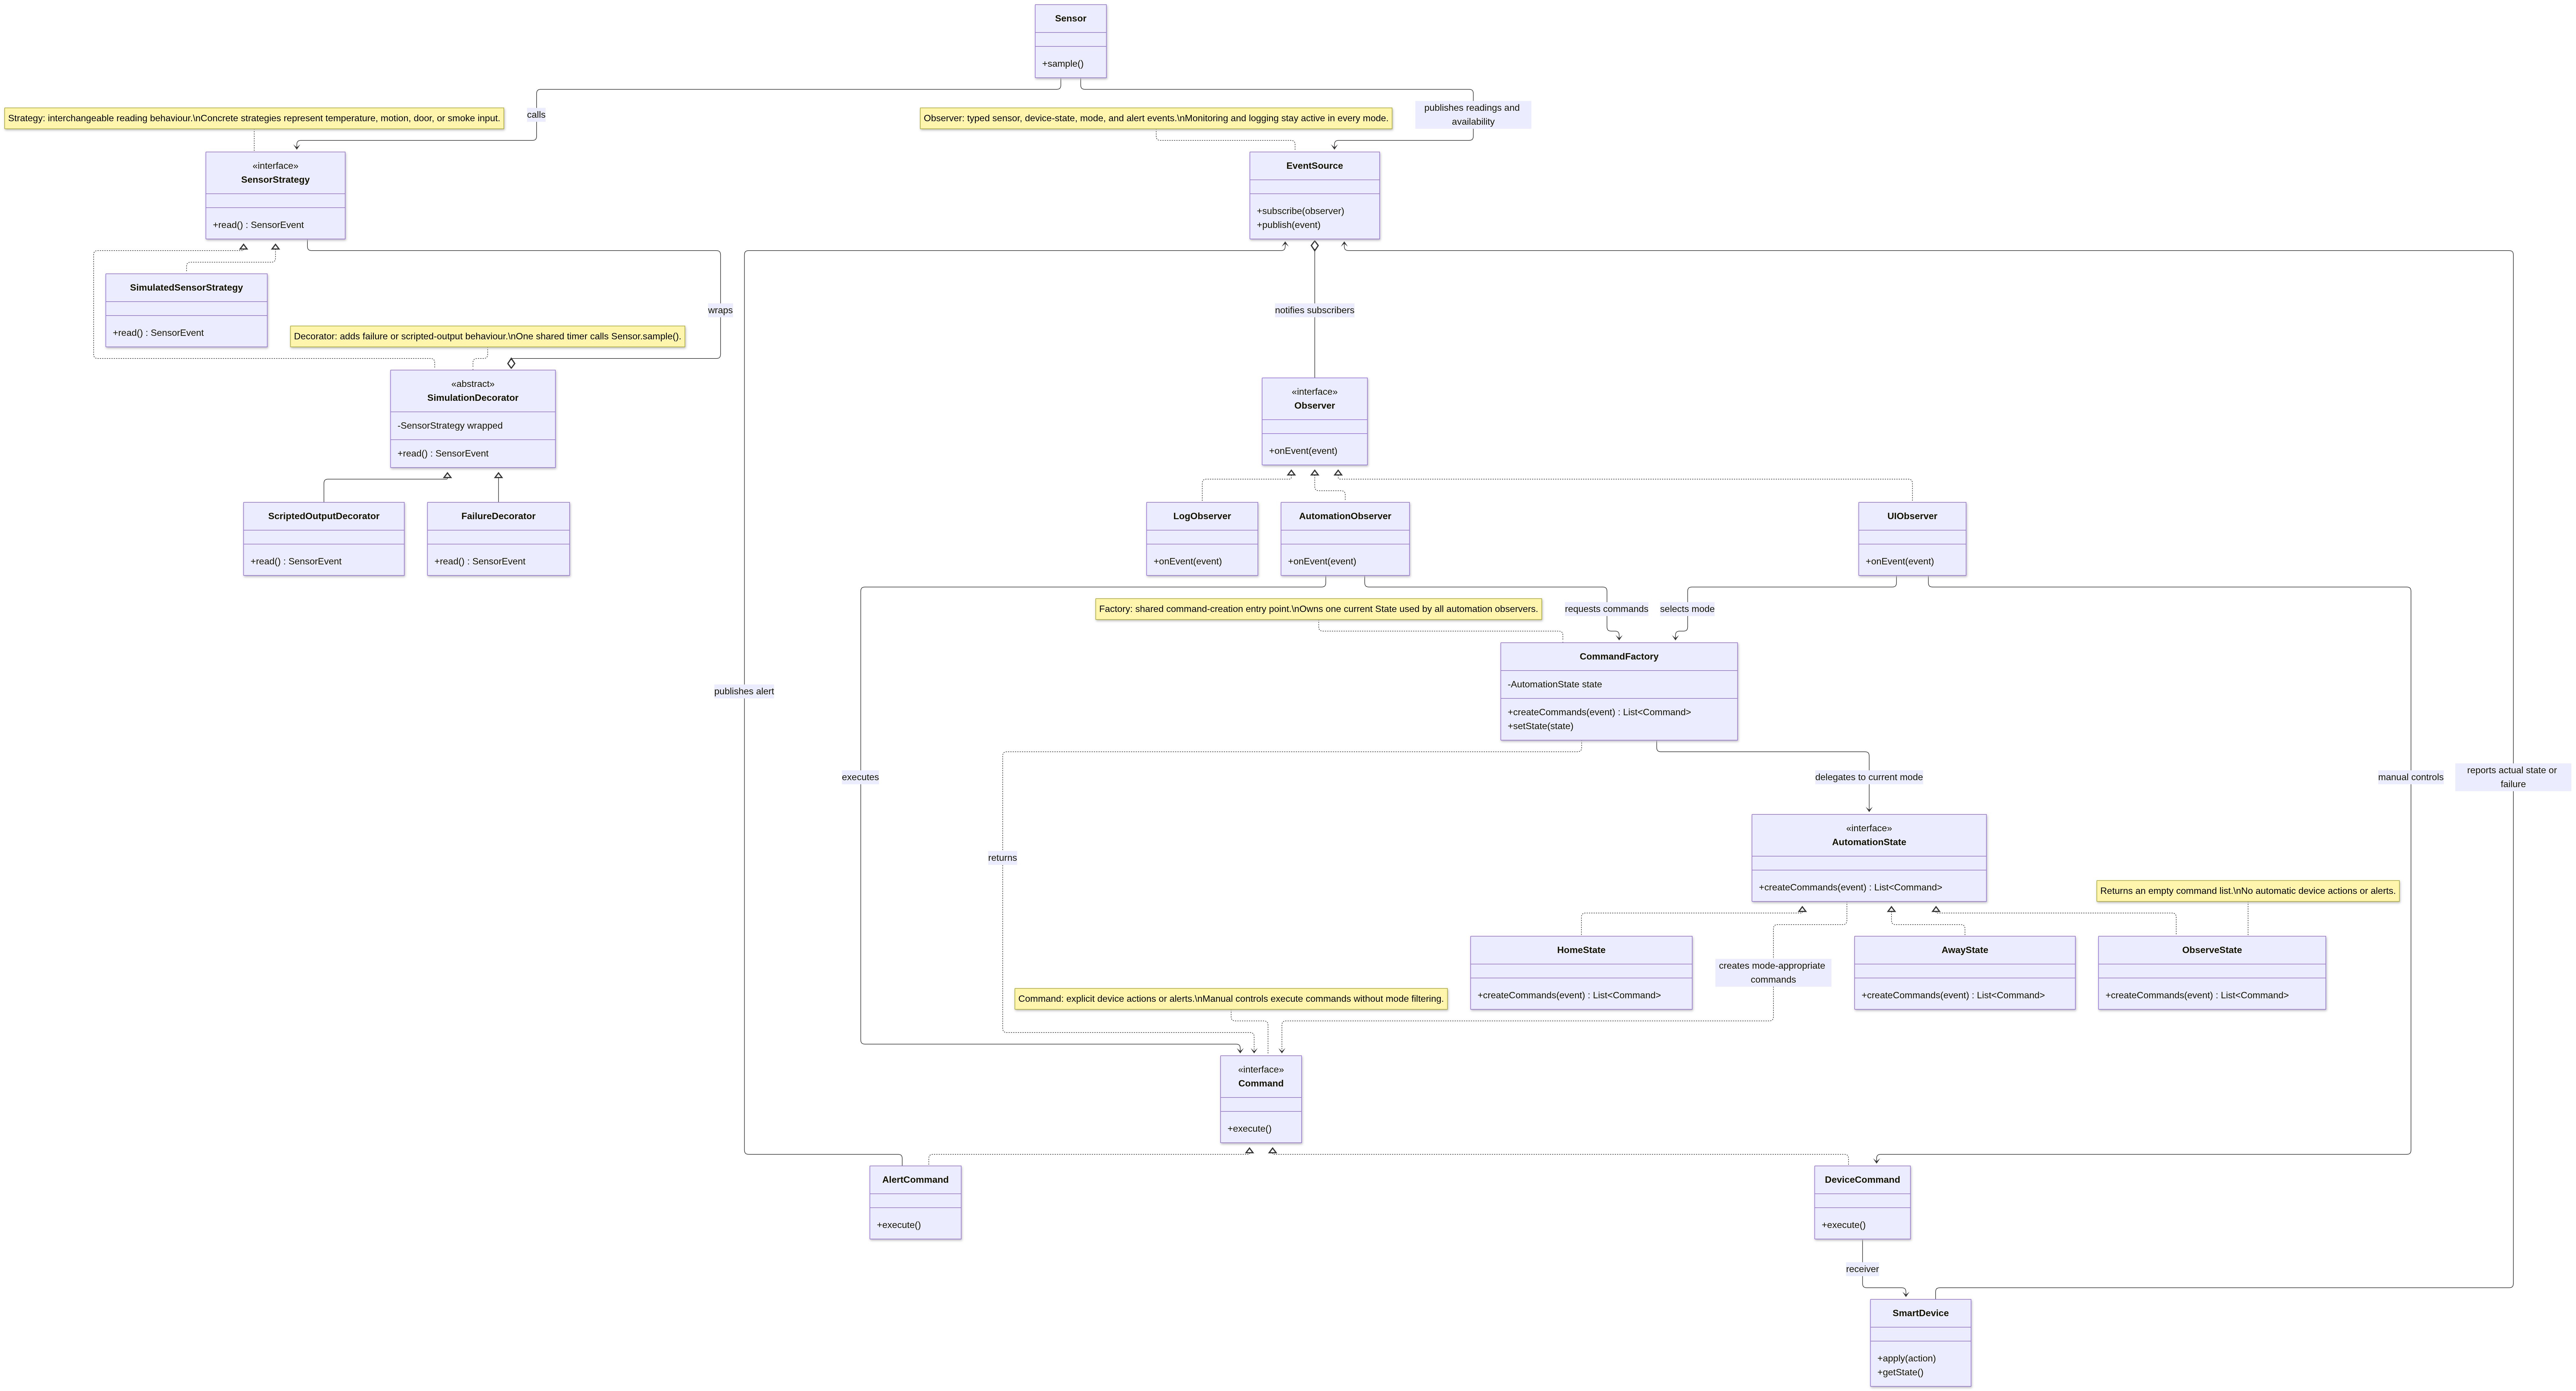
\includegraphics[width=\linewidth]{figures/uml-rev-1.png}
  \caption{Initial HAL class diagram showing Strategy, Decorator, Observer, Factory, State, and Command.}
  \label{fig:hal-class-diagram}
\end{figure}

\subsubsection{Design Patterns and Interactions}
Figure~\ref{fig:hal-activity-diagram} outlines the sensor-to-action flow: a sensor calls its strategy, publishes an event, and notifies observers. The automation observer calls the command factory; the factory calls the current state; and the observer executes the returned commands. Home and Away states select responses appropriate to the event. Observe returns no commands, while monitoring and logging continue. Device commands report actual outcomes, and alert commands publish alerts for the interface and log. The branching event notifications represent subscribers rather than concurrent execution threads.

\begin{figure}[H]
  \centering
  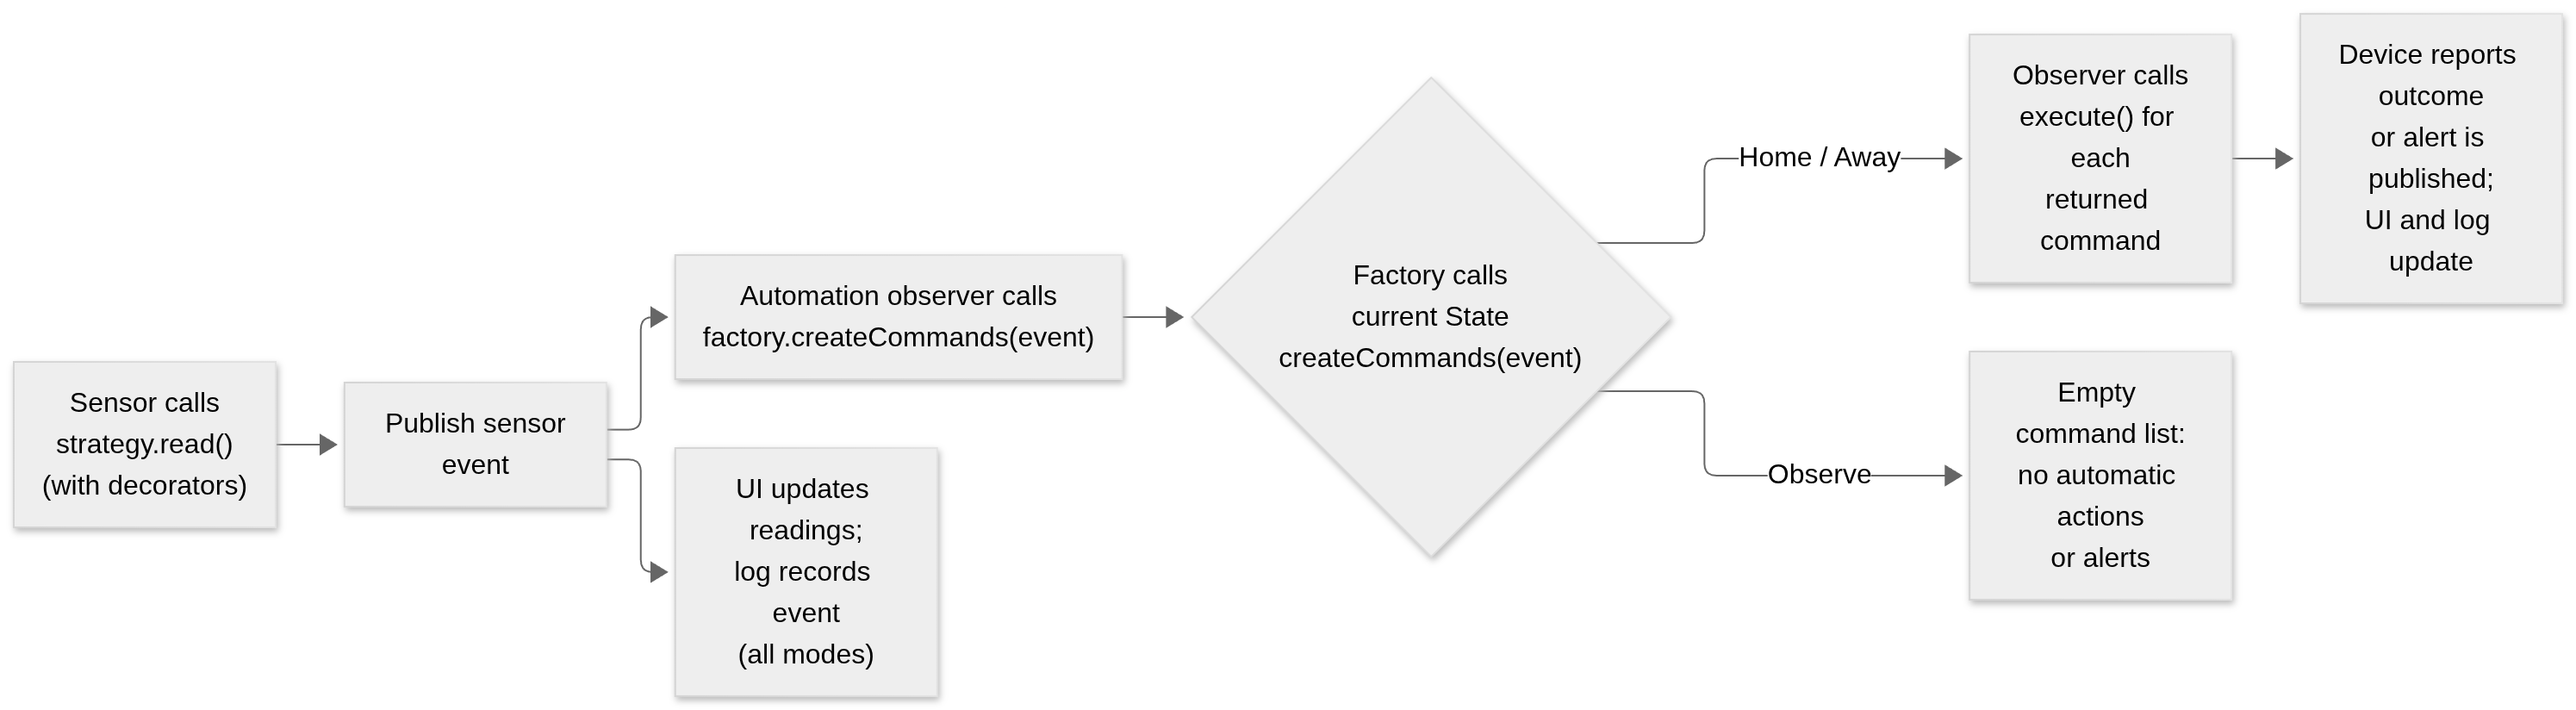
\includegraphics[width=\linewidth,height=0.60\textheight,keepaspectratio]{figures/activity-rev-1.png}
  \caption{HAL activity flow from sensor sampling through mode-dependent command creation and execution.}
  \label{fig:hal-activity-diagram}
\end{figure}

\subsection{Environmental, Societal, Safety, and Economic Considerations}
\templateprompt{Explain how the design addresses relevant environmental, societal, safety, and economic considerations. Discuss privacy, security, ethical issues, and other applicable smart-home challenges, and connect these considerations to the engineering constraints.}

\subsection{Limitations}
\templateprompt{Describe the limitations of the proposed design and, later, the implemented prototype. Explain the limits of software simulation and any unsupported scenarios.}

\chapter{Team Work}
\templateprompt{Record the contributions of both team members, task distribution, and actual project meetings. Replace the placeholders below with real meeting records and add further meetings as needed.}
\meetingtemplate{1}
\meetingtemplate{2}
\meetingtemplate{3}
\meetingtemplate{4}

\chapter{Project Management}
\templateprompt{Provide a Gantt chart showing tasks, progress, and task predecessors. State each task's slack time and identify the critical path. Include the project milestones: deliverable one on October 6, prototype and updated documentation on November 3, midterm report and demo on December 1, and final presentation and technical report on December 8, 2026.}
\placeholderfigure{Insert the project Gantt chart.}{Project schedule and critical path}

\chapter{Conclusion and Future Work}
\templateprompt{Summarize the work completed for the current deliverable. Explain which functions and objectives have been achieved and which constraints have been satisfied. Recommend future improvements based on the design or prototype's limitations.}

% Keep a numbered placeholder until there are actual citations, so the empty
% template compiles without running BibTeX on an empty bibliography.
\ifreportreferences
  \bibliographystyle{ieeetr}
  \bibliography{references}
\else
  \chapter{References}
  \templateprompt{Use IEEE reference style and list only cited sources. Add sources to references.bib and cite them with \texttt{\textbackslash cite\{key\}}. Enable the bibliography using the switch in the preamble; see report/README.md for instructions.}
\fi

\chapter{Appendix}
\templateprompt{Include additional supporting information here. Add sections as needed.}

\end{document}
